% Beamer Presentation and Lecture Note Template
% Version 0.1
% by Paul Vesey

\mode<presentation> {
\usetheme{Antibes}
\setbeamercovered{invisible}
\setbeamertemplate{footline}[frame number]
\setbeamertemplate{navigation symbols}{} 
}

\usepackage{eurosym}
\usepackage{graphicx}
\usepackage{wasysym}
\usepackage{hyperref}
\usepackage{amsmath}
\usepackage{amssymb}
\usepackage{mathtools}
\usepackage{tikz}
\usepackage{pgf}
\usepackage{pgfplots}
\usepackage{pxfonts}
\usepackage{textcomp}
\usepackage{verbatim}
\usepackage{color}
\usepackage{xcolor}
\usepackage{fix-cm}


\author{Paul Vesey}
\institute[TUS]
{
Technological University of the Shannon \\
\medskip
{\emph{paul.vesey@tus.ie}}
}
\date{Autumn 2022}



%
\title[Project Management]{Project Human Resource Management}


\begin{document}
%
\usetikzlibrary{arrows}
\usepgflibrary{patterns}

\tableofcontents
\newpage



\begin{frame}
\titlepage
\end{frame}\begin{center}\line(1,0){250}\end{center}
%
%


\section{Project Human Resource Management}

\subsection{Introduction}



\begin{frame}
\frametitle{Project HRM}
\begin{itemize}
	\item Project HRM includes the processes to organise and manage the Project Team.
	\item The Project Management Team is a subset of the Project Team.
	\item The Project Management Team are responsible for:
		\begin{itemize}
			\item Planning
			\item Controlling
			\item Closing
		\end{itemize}
\end{itemize}
The Project Sponsor works with the Project Management Team.
\end{frame}\begin{center}\line(1,0){250}\end{center}
 
 
\begin{frame}
\frametitle{Project HRM}{The Project HRM processes are:}
\begin{enumerate}
	\item Develop Human Resource Plan
		\begin{itemize}
			\item 		Identifying and documenting project roles, responsibilities, and reporting relationships, as well as creating the staffing management plan
		\end{itemize}
	\item Acquire Project Team
		\begin{itemize}
			\item 		Obtaining the human resources required to complete the project. 
		\end{itemize}
	\item Develop Project Team
		\begin{itemize}
			\item 		Improving Competencies and interactions of team members to enhance project performance
		\end{itemize}
	\item Manage Project Team
		\begin{itemize}
			\item 		Tracking team member performance, providing feedback, resolving issues, and coordinating changes to enhance project performance
		\end{itemize}
\end{enumerate}
\end{frame}\begin{center}\line(1,0){250}\end{center}
 


\subsection{Develop HR Plan}
 
\begin{frame}
\frametitle{Develop Human Resource Plan}
\textbf{Part of the Planning Process Group}
\begin{figure}
	\centering
		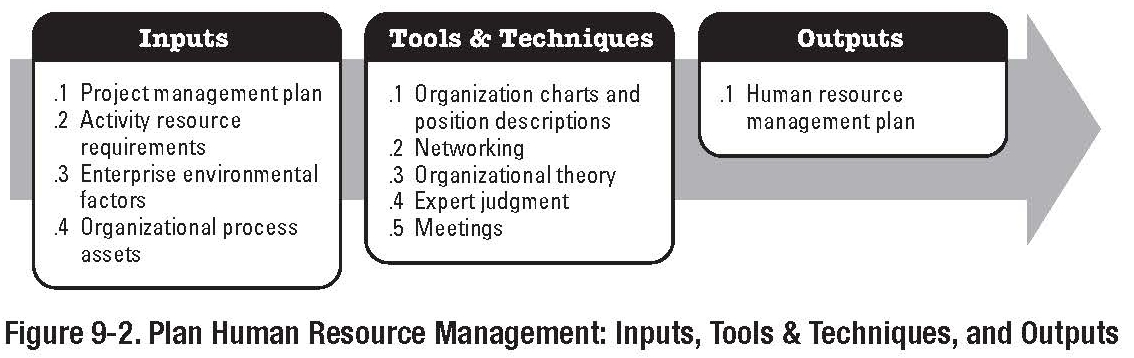
\includegraphics[width = 10cm]{images/Fig9-2.jpg}
	\label{fig:9-2}
\end{figure}
\end{frame}\begin{center}\line(1,0){250}\end{center}

 
\begin{frame}
\frametitle{Develop HR Plan}
HR Planning determines:
\begin{itemize}	
	\item Project Roles
	\item Responsibilities
	\item Reporting Relationships
	\item Staffing Management Plan
\end{itemize}
Project Roles can be for persons or groups\\
Staffing Management Plan typically details when resources will be required and where they will come from - Staff, Contract, Subcontractor, etc.
\end{frame}\begin{center}\line(1,0){250}\end{center}


\begin{frame}
\frametitle{Staffing Management Plan}
\textbf{Records Details of:}
\begin{itemize}
	\item When Resources will be required.
	\item Where they will come from.
		\begin{itemize}	
			\item Staff, Contract, Subcontractor, etc.
		\end{itemize}	
	\item Criteria for release from the project.
			\begin{itemize}	
				\item Deliverables achieved, Project Complete, Task Complete, etc.
			\end{itemize}	
	\item Training Needs.
			\begin{itemize}	
				\item Will resources require specific training before embarking on the project?
			\end{itemize}	
	\item Other Criteria.
			\begin{itemize}	
				\item Background checks?
			\end{itemize}	
\end{itemize}
\end{frame}\begin{center}\line(1,0){250}\end{center}
 
 
\begin{frame}
\frametitle{Staffing Management Plan}
\textbf{Records Details of:}
\begin{itemize}
	\item Plans for Recognition and Reward.\\
	\item Safety Issues.\\
	\item Impact of the Staffing Management Plan on the Organisation.\\
			\begin{itemize}
				\item Critical for SME's.  If all resources are being tied up on one project, then how does this effect other projects?
			\end{itemize}
\end{itemize}
\end{frame}\begin{center}\line(1,0){250}\end{center}


\begin{frame}
\frametitle{Develop HR Plan \hfill\hfill Inputs}
\textbf{Enterprise Environmental Factors:}
\begin{itemize}
	\item Organisational
		\begin{itemize}
			\item Which Departments? What are their working arrangements? What formal or informal relationships do they have? 
		\end{itemize}
	\item Technical
		\begin{itemize}
			\item What disciplines are needed for the project?
			\item Systems Engineering? 
		\end{itemize}
	\item Interpersonal
		\begin{itemize}
			\item Reporting relationships; Supplier-Customer Relationships; Cultural issues?; Trust and Respect..
		\end{itemize}
	\item Logistical
		\begin{itemize}
			\item Where are people in relation to each other and the work?
		\end{itemize}
	\item Political
		\begin{itemize}
			\item Individual and Group Politics
			\item A good PM is usually a politician, whether they like it or not.. \smiley
		\end{itemize}
\end{itemize}
\end{frame}\begin{center}\line(1,0){250}\end{center}
 
 
\begin{frame}
\frametitle{Develop HR Plan \hfill\hfill Inputs}
\textbf{Enterprise Environmental Factors (cont)}
\begin{itemize}
	\item Organisational Structure
	\begin{itemize}
		\item Functional, Weak Matrix, Strong Matrix, etc.
		\item Refer to early lectures  
	\end{itemize}
	\item Collective Bargaining Agreements
	\begin{itemize}
		\item Contractual agreements with Unions or other employees.
		\item Will there be issues of Demarcation?
	\end{itemize}
	\item Economic Conditions
	\begin{itemize}
		\item Internal; Training Fund; Recruitment Freeze (HSE since September '07)
		\item External; Competition, Economic Environment, etc.
	\end{itemize}
\end{itemize}
\end{frame}\begin{center}\line(1,0){250}\end{center}
 
 
\begin{frame}
\frametitle{Develop HR Plan \hfill Inputs}
\textbf{Organisational Process Assets}
\begin{itemize}
	\item Historical Information - Lessons Learned
	\item Templates
	\begin{itemize}
		\item Organisation Structures 
		\item Job Descriptions
		\item Performance Appraisals 
		\item Employee Voice Systems
		\item Conflict Management Systems
	\end{itemize}
	\item Checklists
	\begin{itemize}
		\item Typical Competencies
		\item Safety Considerations, Tax Clearance Certs, etc.
		\item Safe Pass
		\item Insurance
		\item Vetting (South Midland Construction)
	\end{itemize}
\end{itemize}
\end{frame}\begin{center}\line(1,0){250}\end{center}
 
 
\begin{frame}
\frametitle{Develop HR Plan \hfill Inputs}
\textbf{Activity Resource Requirements:}\\
Resource Type and Quantity can be determined from:
\begin{itemize}
	\item WBS
	\item Parametric Estimating
	\item Etc.
\end{itemize}
\end{frame}\begin{center}\line(1,0){250}\end{center}


\begin{frame}
\frametitle{Develop HR Plan \hfill Tools and Techniques}
\textbf{Organisational Charts and Position Descriptions.}\\
Typically 3 types:\\
\begin{figure}
	\centering
		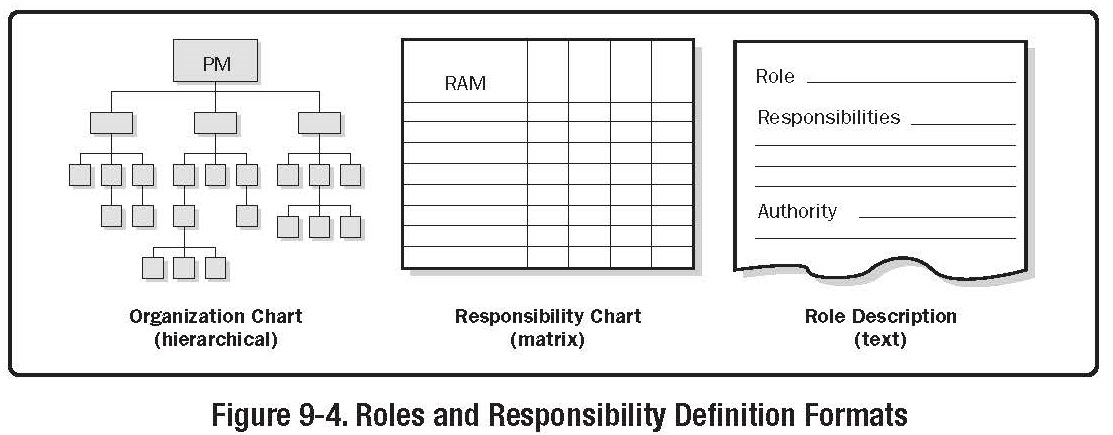
\includegraphics[width = 10cm]{images/Fig9-4.jpg}
	\label{fig:9-4}
\end{figure}
\end{frame}\begin{center}\line(1,0){250}\end{center}


\begin{frame}
\frametitle{Develop HR Plan}
\textbf{Hierarchical-Type}
	\begin{itemize}
		\item Typical Organisational Chart
	\end{itemize}
\textbf{Organisational Breakdown Structure}
	\begin{itemize}
		\item Top-Down Format	
		\item Those at the bottom tend not to like it..
	\end{itemize}
\textbf{Resource Breakdown Structure}	
	\begin{itemize}
		\item Breaks down resources according to skills and competencies
	\end{itemize}
\end{frame}\begin{center}\line(1,0){250}\end{center}
 
 
\begin{frame}
\frametitle{Organisational Breakdown Structure}
\begin{figure}
	\centering
		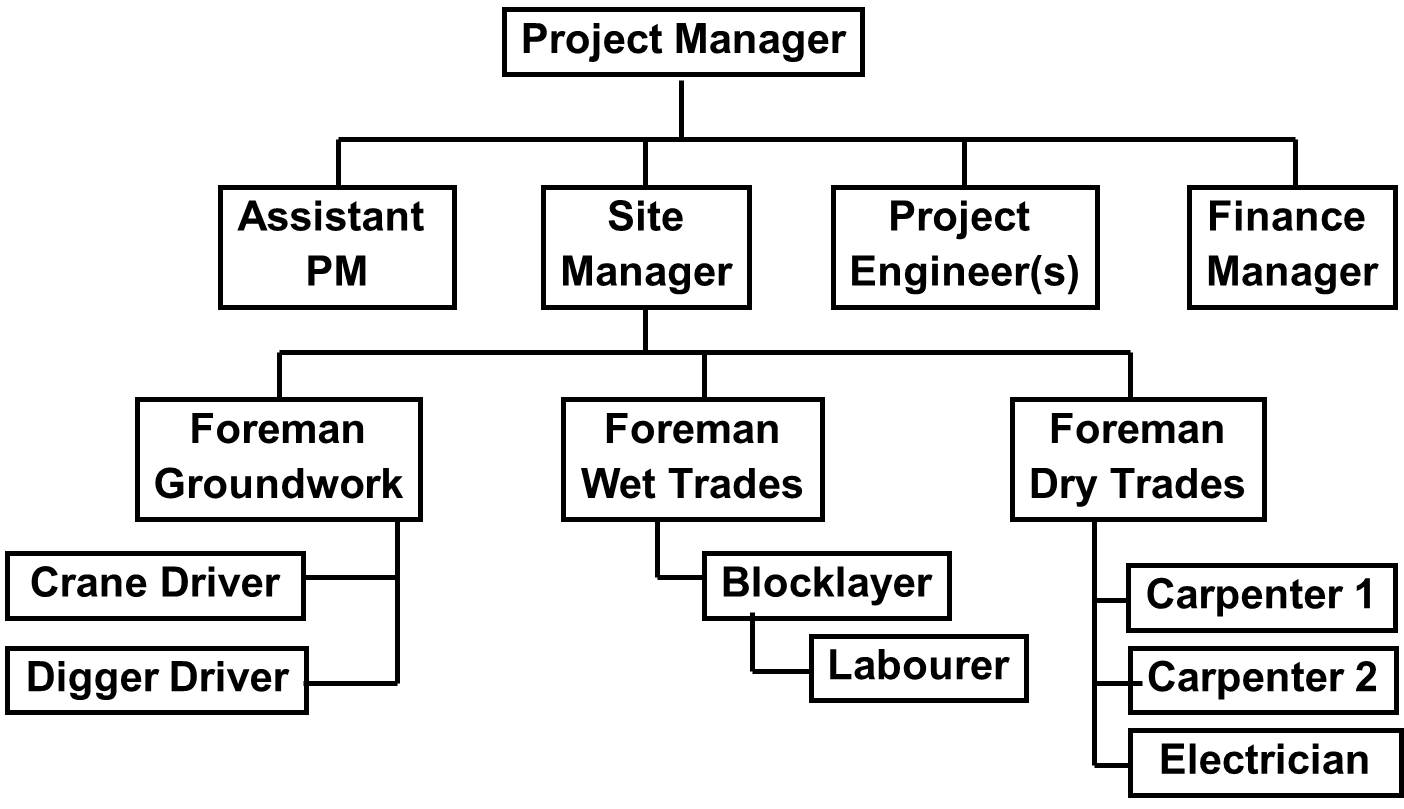
\includegraphics[width = 10cm]{images/obs.jpg}
	\label{fig:obs}
\end{figure}
\end{frame}\begin{center}\line(1,0){250}\end{center}


\begin{frame}
\frametitle{Resource Breakdown Structure}
\begin{figure}
	\centering
		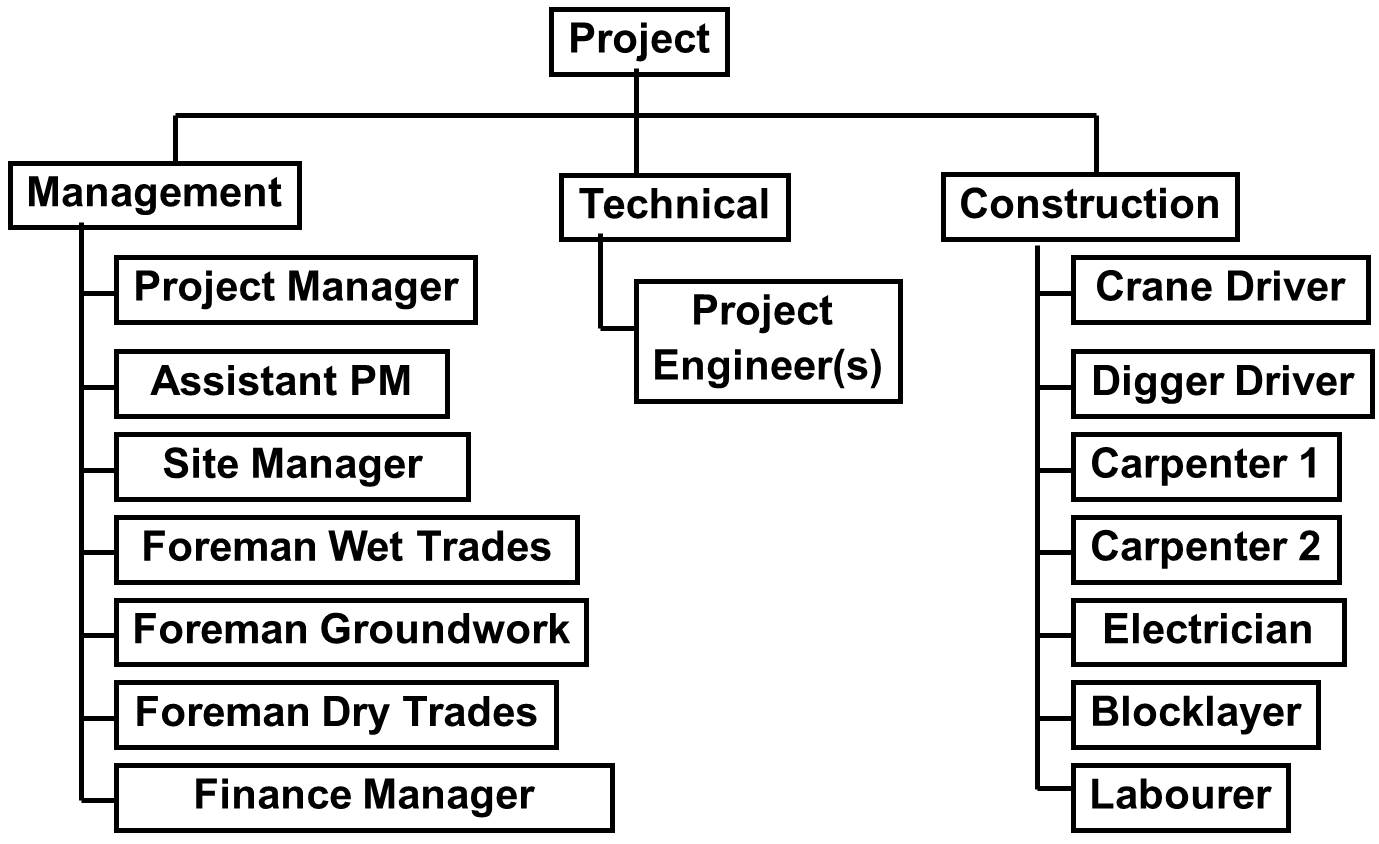
\includegraphics[width = 10cm]{images/rbs.jpg}
	\label{fig:rbs}
\end{figure}
\end{frame}\begin{center}\line(1,0){250}\end{center}
 
 
\begin{frame}
\frametitle{RBS and Project Management Software}
\begin{itemize}
	\item More sophisticated PM Software, such as Primavera and MS Project Server will include RBS functionality.
	\item Note that Standard MS Project does not include RBS functionality
\end{itemize}
\begin{figure}
	\centering
		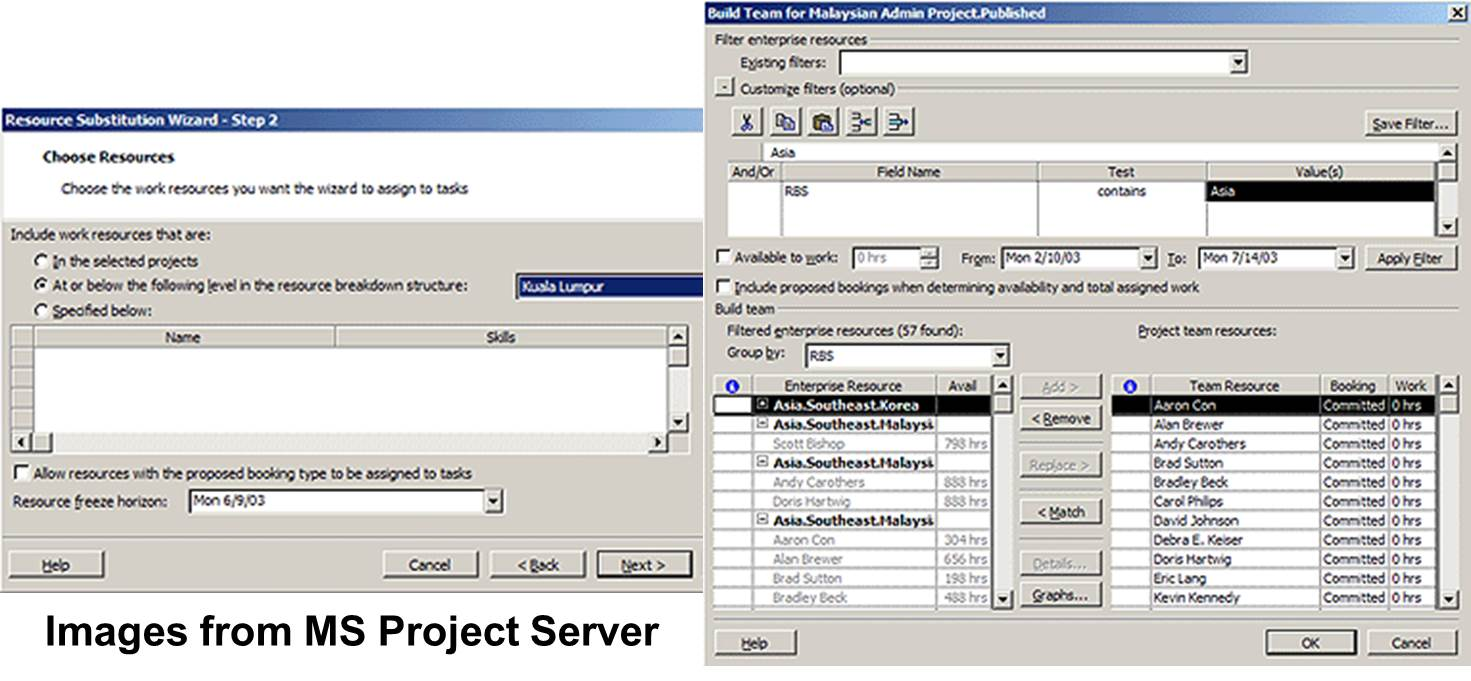
\includegraphics[width = 10cm]{images/prjserver.jpg}
	\label{fig:msprojserver}
\end{figure}
\end{frame}\begin{center}\line(1,0){250}\end{center}


\begin{frame}
\frametitle{RBS - Further Information}
\textbf{RBS (MS Project Server)}\\
Databases allow greater information to be stored:\\
\begin{itemize}
	\item Skills
	\item Availability
	\item Location
	\item Responsibility Level
	\item Etc.
\end{itemize}
\end{frame}\begin{center}\line(1,0){250}\end{center}
 
 
\begin{frame}
\frametitle{Matrix Charts}
\textbf{Responsibility Assignment Matrix}
\begin{itemize}
	\item Illustrates the connection between the work required from the WBS and who will be responsible for it from the OBS or RBS
\end{itemize}
\begin{figure}
	\centering
		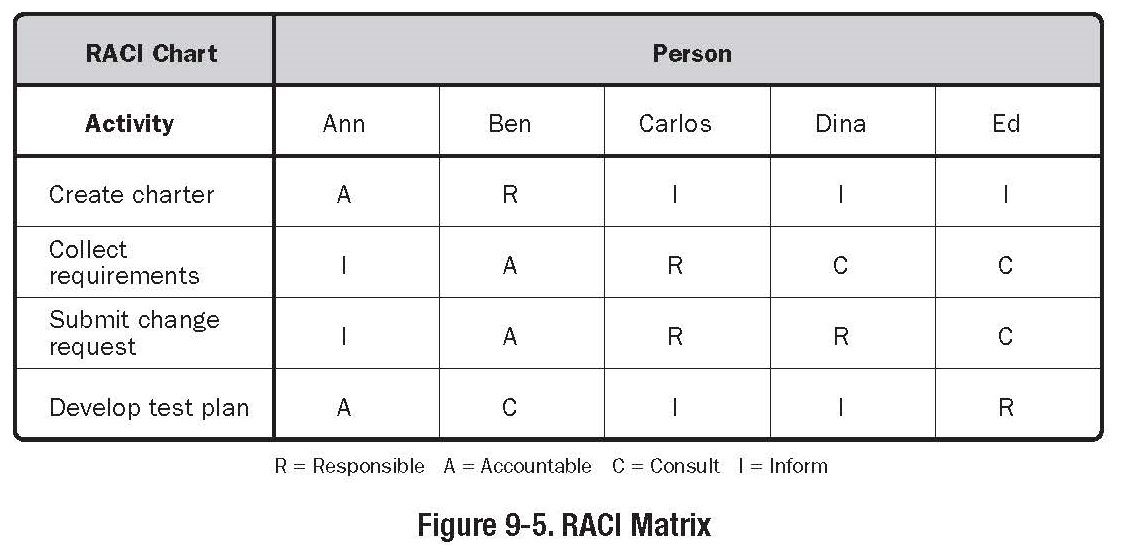
\includegraphics[width = 10cm]{images/Fig9-5.jpg}
	\label{fig:9-5a}
\end{figure}
\end{frame}\begin{center}\line(1,0){250}\end{center}
 
 
\begin{frame}
\frametitle{Matrix Charts}
\textbf{RACI Responsibility Assignment Matrix}
\begin{itemize} 
	\item Responsible - Responsible for Task
	\item Accountable - To whom `R' is Accountable
	\item Consult - Has capability and/or information necessary to perform the work
	\item Inform - Must be notified of results, but does not need to be consulted
\end{itemize}
\begin{figure}
	\centering
		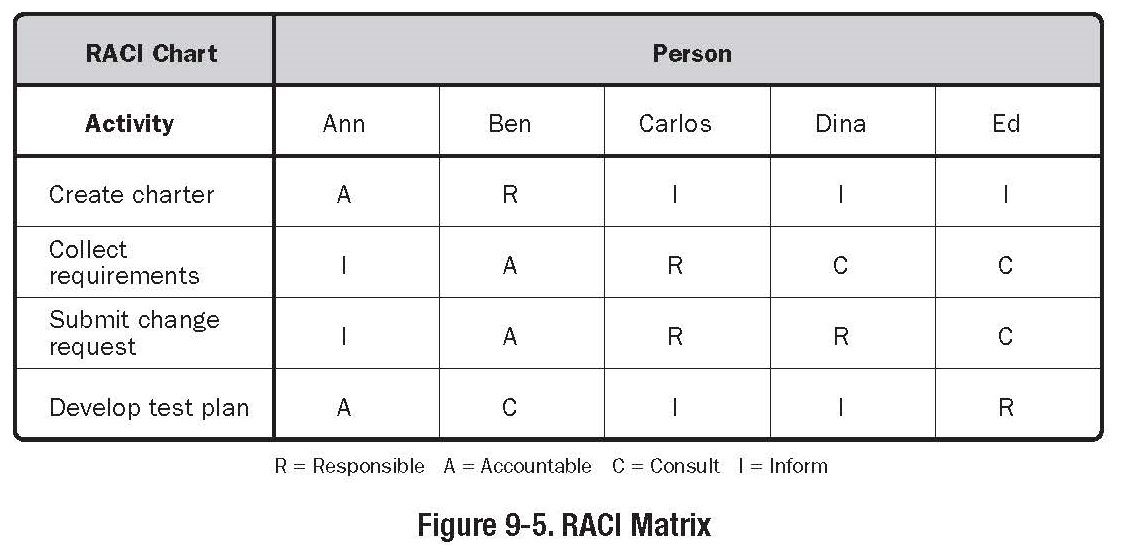
\includegraphics[width = 6cm]{images/Fig9-5.jpg}
	\label{fig:9-5b}
\end{figure}
\end{frame}\begin{center}\line(1,0){250}\end{center}


\begin{frame}
\frametitle{}
\textbf{Typical Process to Generate an RACI Chart:}
\begin{enumerate}
	\item Identify all of the activities involved in the project (WBS!)
	\item Identify all roles necessary to complete the project.
	\item Identify who will satisfy R, A, C, I for each task
		\begin{itemize}
			\item In general only one person or group should be assigned as `Responsible'
		\end{itemize}
	\item Resolve overlaps and gaps
		\begin{itemize}
			\item Overlap; more than one R
			\item Gap; no R, no A, etc.
		\end{itemize}
\end{enumerate}	
\end{frame}\begin{center}\line(1,0){250}\end{center}
 
 
\begin{frame}
\frametitle{Develop HR Plan \hfill Tools and Techniques}
\textbf{Organisation Charts and Position Descriptions}
\begin{itemize}
	\item Text Orientated Formats
			\begin{itemize}
				\item Usually an outline form.
				\item Provides information such as responsibility, authority, competencies, and qualifications.
				\item Good for capturing lessons learned information.
				\item Networking
			\end{itemize}
\end{itemize}
\textbf{Organisation Theory}
		\begin{itemize}
			\item Information regarding the ways people, teams and organisational units behave such as the Hawthorne Studies, Maslow, Theory X-Theory Y, etc.
		\end{itemize}
\end{frame}\begin{center}\line(1,0){250}\end{center}
 
The Hawthorn Effect or Observer Effect are terms used to describe how people will modify their behavior when being observed.  The Hawthorn Studies were commissioned by Western Electric of Chicago between 1924 and 1932.  One of the objectives of the study was to determine how light levels effected worker performance.  A simple hypothesis was formed: more light, better work.  However, when conducting the studies it was found that the opposite occurred.  As light levels dropped, performance improved. This remained until a point was reached where performance cratered.  Later, it was determined that the results observed were attributable workers reacting to being watched and questioned about their work. \\

Another interesting phenomenon is the the Pygmalion or Rosenthal Effect, whereby the greater the expectation, the greater a person will perform.  The opposite effect is the golem effect whereby low expectations generally yield low performance. 


 
\begin{frame}
\frametitle{Develop HR Plan \hfill Outputs}
\textbf{Human Resource Plan}\\
\textbf{Roles and Responsibilities}\\
	\begin{itemize}
		\item Role
		\item Authority
		\item Responsibility
		\item Competency
	\end{itemize}
\textbf{Project Organisation Charts}\\
\textbf{Staffing Management Plan}\\
	\begin{itemize}
		\item Staff Acquisition
		\item Timetable
		\item Release Criteria
		\item Training Needs
		\item Recognition and Rewards
		\item Compliance and Safety
	\end{itemize}
\end{frame}\begin{center}\line(1,0){250}\end{center}
 
 

%% END OF LECTURE SLIDE
\begin{frame}
\frametitle{Next Lecture \hfill Reading:}
`A Guide to the Project Management Body of Knowledge'\\ 
Chapter 9
\begin{figure}[h]
	\centering
		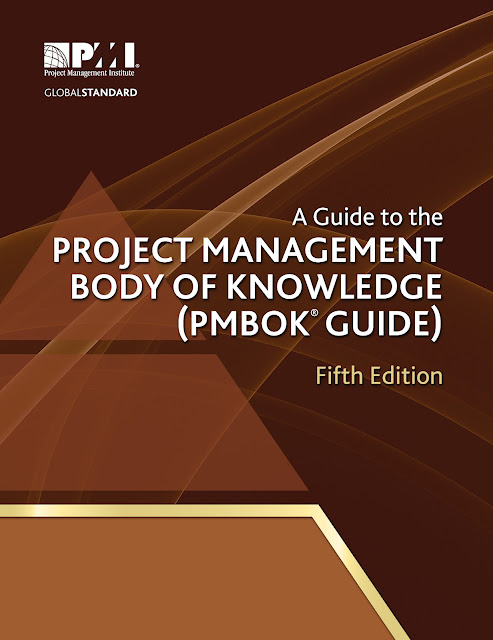
\includegraphics[width = 4cm]{images/book.jpg}
\end{figure}
\end{frame}\begin{center}\line(1,0){250}\end{center}
%% END OF LECTURE SLIDE
\subsection{HR Planning}


 
\begin{frame}
\frametitle{HR Planning Outputs}
\textbf{Roles and Responsibilities}
\begin{itemize}
	\item Role: Label describing the portion of the project for which an individual is responsible
	\item Authority: Authority to apply project resources, make decisions, and sign approvals
	\item Responsibility: Work that a PM team member is expected to perform in order to complete the project's activities
	\item Competency: Skill and Capacity required to complete project objectives
\end{itemize}
\end{frame}\begin{center}\line(1,0){250}\end{center}


\begin{frame}
\frametitle{HR Planning Outputs}
\begin{block}{Responsibility and Authority are not the same thing}
Individuals will perform best when they responsibility and authority are matched.
\end{block}
Responsibility / Authority miss-match is very common.  How many times have you experienced either:
\begin{itemize}
	\item Someone's decision/instructions being reversed or changed? 
	\item Someone having to constantly respond with `I need approval from X before I can give you the go-ahead'
\end{itemize}
\end{frame}\begin{center}\line(1,0){250}\end{center}
 
 
\begin{frame}
\frametitle{HR Planning Outputs}
\textbf{Project Organisation Charts}
\begin{itemize}
	\item Graphic Representation of project team members and their reporting relationships which are usually included in H\&S Plan, Quality Plans, etc.
\end{itemize}
\begin{figure}
	\centering
		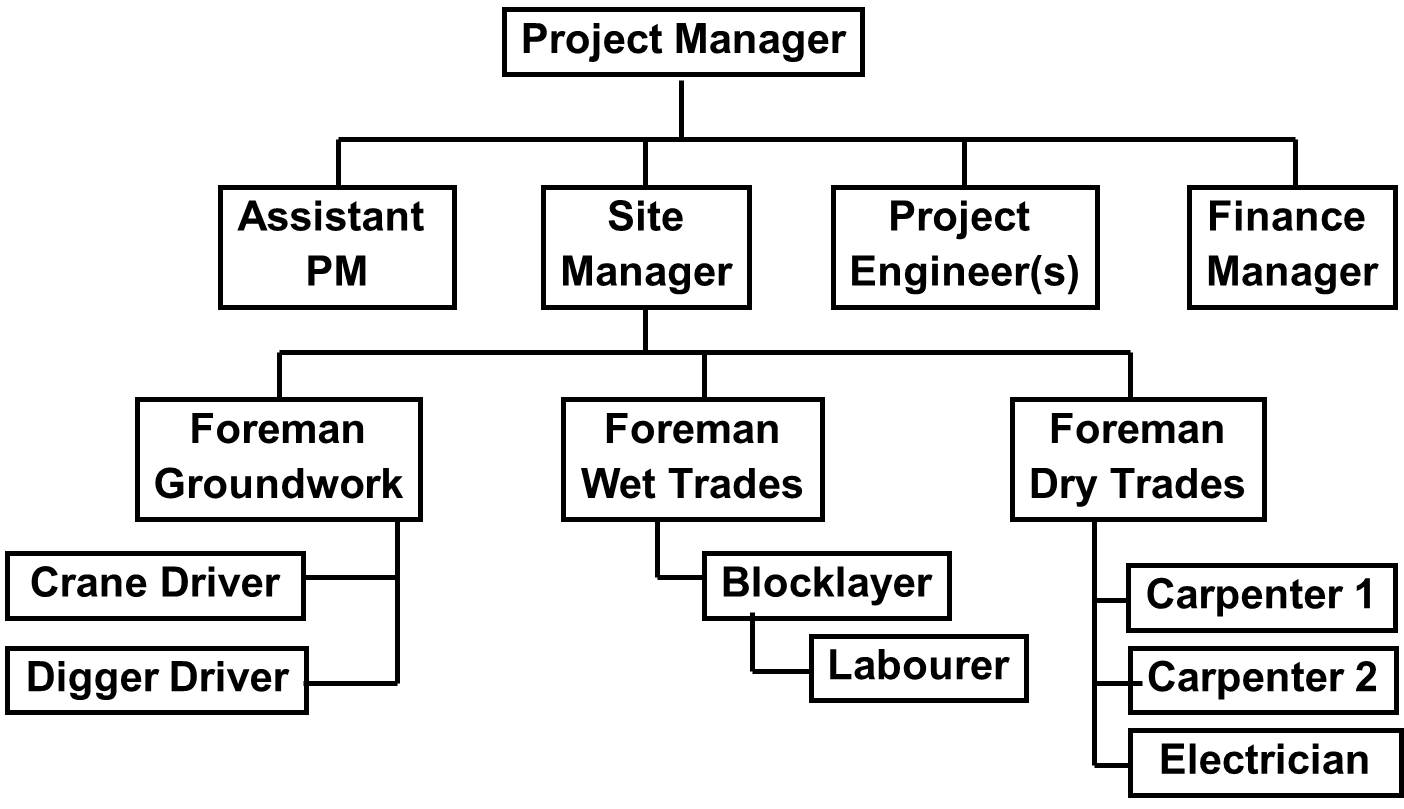
\includegraphics[width = 4cm]{images/obs.jpg}
	\label{fig:obs2}
\end{figure}
\end{frame}\begin{center}\line(1,0){250}\end{center}




\begin{frame}
\frametitle{HR Planning Outputs \hfill Staffing Management Plan}
\textbf{Staff Acquisition:}
\begin{itemize}
	\item Where will staff come from; Subcontract, Direct Staff, Contract Staff
	\item Proximity; Do staff need to be in the same location? Not always the case; does QS or Engineer need to be on site all, day every day?
	\item HR Department; Can HR Department assist in staffing the project?
	\item Timetable;	When will staff be required. When will acquisition (recruitment) have to start in order to meet requirements?
\end{itemize}
\end{frame}\begin{center}\line(1,0){250}\end{center}
 
 
\begin{frame}
\frametitle{HR Planning Outputs \hfill Staffing Management Plan}
\textbf{Release Criteria:}
		\begin{itemize}
			\item Method and Timing for release of staff.
		\begin{itemize}
			\item Method: Milestone, Time based, Task based, etc.
			\item Timing: Need to consider how individuals are transferred to other projects.
		\end{itemize}
		\end{itemize}
\textbf{Training Needs:}
		\begin{itemize}
			\item  	What training staff will be required to undertake
		\end{itemize}
\textbf{Recognition and Rewards:}
		\begin{itemize}
			\item  	Clear reward structure; ideally aligned with the individuals  performance on the project
		\end{itemize}
\textbf{Compliance:}
\begin{itemize}
	\item Strategies to comply with Government Regulations
			\begin{itemize}
				\item Construction Worker Pension Scheme (Supreme Court Ruling 9th May 2013)
			  	\item Safety Policies and Procedures that protect staff from hazards
			\end{itemize}
 	\item Also included in H\&S Plan, and Risk Register
\end{itemize}
\end{frame}\begin{center}\line(1,0){250}\end{center}

Taken from the CWPS website 18-7-2013.\\ 
\href{http://www.cwps.ie/news/default.aspx?iid=43}{http://www.cwps.ie/news/default.aspx?iid=43}

\begin{figure}[htbp]
	\centering
		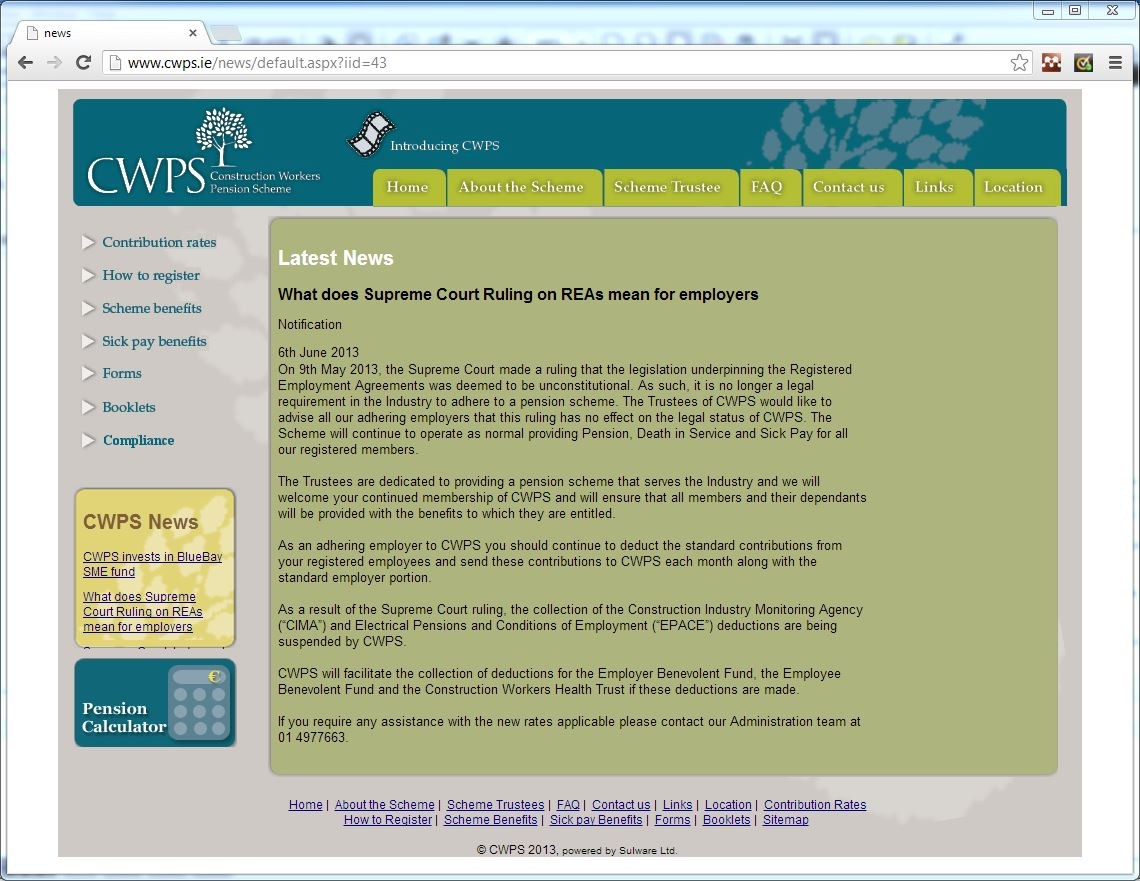
\includegraphics[width=14cm]{images/CWPS.JPG}
	\caption{CWPS Screen Shot}
	\label{fig:CWPS}
\end{figure}











\begin{frame}
\frametitle{Resource Histogram}
\begin{itemize}
	\item Details quantity and timing of resources.
	\item Does not detail skill level.
\end{itemize}
\begin{figure}
	\centering
		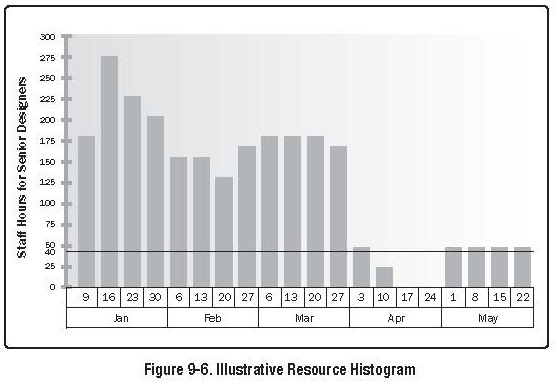
\includegraphics[width = 7cm]{images/Fig9-6.jpg}
	\label{fig:9-6}
\end{figure}
\end{frame}\begin{center}\line(1,0){250}\end{center}


\begin{frame}
\frametitle{Acquire Project Team \hfill Part of the Planning Process Group}
\begin{figure}
	\centering
		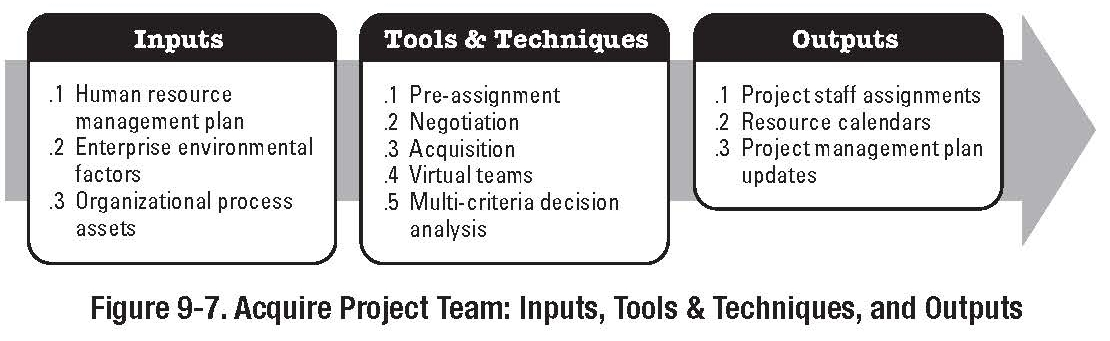
\includegraphics[width = 10cm]{images/Fig9-7.jpg}
	\label{fig:9-7}
\end{figure}
\end{frame}\begin{center}\line(1,0){250}\end{center}
 
 
\begin{frame}
\frametitle{Acquire Project Team \hfill Inputs}
\textbf{Process of obtaining the resources required to complete the project}\\
Enterprise Environmental Factors:
\begin{itemize}
	\item Availability
	\item Ability
	\item Experience
	\item Interests
	\item Cost
\end{itemize}
\end{frame}\begin{center}\line(1,0){250}\end{center}
 
 
\begin{frame}
\frametitle{Acquire Project Team \hfill Inputs}
\textbf{Organisational Process Assets}
\begin{itemize}
	\item HR Department
	\item Policies and Procedures in relation to staff; Disciplinary procedures, Annual Leave, etc.
\end{itemize}
\textbf{Roles and Responsibilities}
\begin{itemize}
	\item Definition of positions, competencies, skills etc.
\end{itemize}
\textbf{Project Organisation Chart}
\begin{itemize}
	\item Refer to book and earlier notes
\end{itemize}
\textbf{Staffing Management Plan}
\begin{itemize}
	\item Refer to book and earlier notes
\end{itemize}
\end{frame}\begin{center}\line(1,0){250}\end{center}
 
 
\begin{frame}
\frametitle{Acquire Project Team \hfill Tools and Techniques}
\textbf{Pre-Assignment:}
\begin{itemize}
	\item Team Members, particularly senior staff, may have been allocated to the project at tender stage, and/or may have been a included as part of the tender proposal.\\
	\begin{itemize}
		\item Very common on Construction Projects; Usual get-out is a provision somewhere in the tender that states that the staff are `indicative'.  
		\item Need to be very careful; can lead to a tender being deemed non-compliant.
	\end{itemize}
\end{itemize}
\end{frame}\begin{center}\line(1,0){250}\end{center}
 
 
\begin{frame}
\frametitle{Acquire Project Team \hfill Tools and Techniques}
\textbf{Negotiations}
\begin{itemize}
	\item Organisation Structure;
	\begin{itemize}
		\item Functional organisation; PM will have to negotiate with Functional Managers in order to obtain staff.
		\item Competition from other PM teams within the organisation.
	\end{itemize}
\end{itemize}
\textbf{Acquisition}
	\begin{itemize}
		\item Source resource from outside organisation: Recruit; Hire Consultant; etc.
	 	\item Virtual Teams: Groups of people with shared goals who fulfil their roles with little or no time spent meeting face to face. Most Construction Contract Management Teams.
	\end{itemize}
\end{frame}\begin{center}\line(1,0){250}\end{center}
 
 
\begin{frame}
\frametitle{Acquire Project Team \hfill Outputs}
\textbf{Project Staff Assignments}
		\begin{itemize}
			\item Project is staffed when appropriate people have been assigned to work on it.
		\end{itemize}
\textbf{Resource Availability}
		\begin{itemize}
			\item Documents the time period that each team member can work on the project.
			\item Very difficult in most environments; often availability issues lead to project delays.
		\end{itemize}
\textbf{Staffing Management Plan (Updates)}
		\begin{itemize}
			\item People seldom fit the original requirements profiles.
			\item Usually the Plan will have to be modified to fit with individuals
			\item Over the course of the project individuals may leave the project unexpectedly; promotion, annual leave, resignation, etc.
		\end{itemize}
\end{frame}\begin{center}\line(1,0){250}\end{center}
 


 
\begin{frame}
\frametitle{Develop Project Team}
\textbf{Part of the Executing Process Group}
\begin{figure}
	\centering
		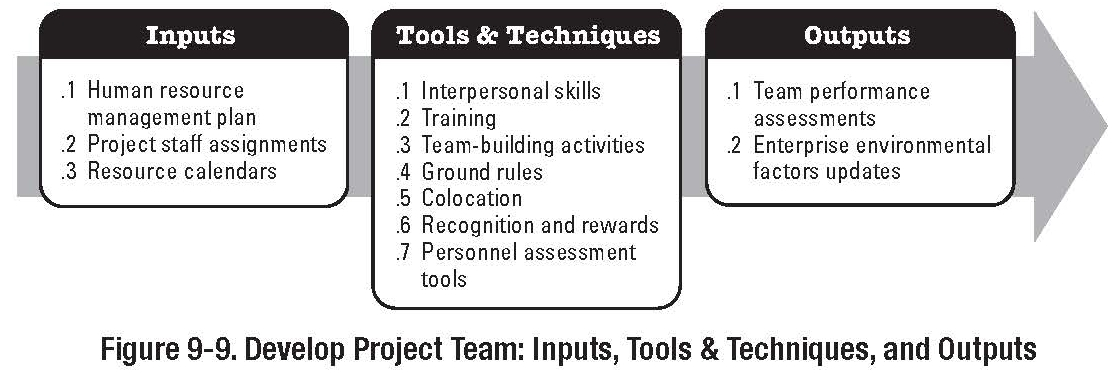
\includegraphics[width = 10cm]{images/Fig9-9.jpg}
	\label{fig:9-9}
\end{figure}
\end{frame}\begin{center}\line(1,0){250}\end{center}


 
 
\begin{frame}
\frametitle{Develop Project Team \hfill Objectives:}
\begin{itemize}
	\item Improve skills of Team Members.
	\item Improve feelings of trust and cohesiveness among team members.
			\begin{itemize}
				\item Construction Sector is notoriously bad at this, evidenced by the levels of conciliation, arbitration, etc.
			\end{itemize}
	\item Best accomplished at the start of the project
\end{itemize}

\begin{block}{Group Dynamics\hfill\textit{Bruce Tuckman 1965}}
	\begin{enumerate}
		\item Forming; coming together
		\item Storming; unsettled, team members vie for position
		\item Norming; team members adjust and moderate
		\item Performing; team gets work done
		\item Mourning; completion of task and break-up of team
	\end{enumerate}
\end{block}
\end{frame}\begin{center}\line(1,0){250}\end{center}


\begin{frame}
\frametitle{Develop Project Team \hfill Inputs}
\textbf{Project Staff Assignments}
\begin{itemize}
	\item List of team members
\end{itemize}
\textbf{Staffing Management Plan}
\begin{itemize}
	\item Refer to book an previous notes
\end{itemize}
\textbf{Resource Calendar}
\begin{itemize}
	\item Resource availability information
\end{itemize}
\end{frame}\begin{center}\line(1,0){250}\end{center}
 
 
\begin{frame}
\frametitle{Develop Project Team \hfill Tools and Techniques}
\textbf{General Management Skills}
\begin{itemize}
	\item Soft Skills
 	\begin{itemize}
		\item Interpersonal Skills
			\begin{itemize}
				\item Understanding sentiments of project team
				\item Listening to what is being said
				\item Understanding the individual circumstances of team members
				\item Anticipating Likely reactions
			\end{itemize}
	\end{itemize}
\end{itemize}
\end{frame}\begin{center}\line(1,0){250}\end{center}
 
 
\begin{frame}
\frametitle{Develop Project Team \hfill Tools and Techniques}
\textbf{Training}
\begin{itemize}
	\item Training Activities designed to enhance the competencies of team members
	\item Mentoring \& Coaching becoming more popular
\end{itemize}
\textbf{Team Building Exercises}
\begin{itemize}
	\item On-site / Offsite / formal / informal
	\item Designed to improve interpersonal relationships by shared experience
	\item Needs to be treated with care; 4WD day; what if someone can't drive?
\end{itemize}
\end{frame}\begin{center}\line(1,0){250}\end{center}




\begin{frame}
\frametitle{Develop Project Team \hfill Tools and Techniques}
\textbf{Ground Rules}
	\begin{itemize}
		\item Clear expectation regarding individual team behaviour and expectations
	\end{itemize}
\textbf{Co-Location}
	\begin{itemize}
		\item Locating team members in the same place to enhance team performance
			\begin{itemize}
				\item Not always practical for construction work.
				\item International construction companies often locate staff in `ex-pat' compounds.  
				\item Recognition and Rewards
			\end{itemize}
	\end{itemize}
\textbf{Recognizing and Rewarding desirable behaviour}
		\begin{itemize}
			\item Needs to be treated with care; refer to book
		\end{itemize}
\end{frame}\begin{center}\line(1,0){250}\end{center}
 


 
\begin{frame}
\frametitle{Develop Project Team \hfill Outputs}
\textbf{Team Performance Assessment}\\
Measures of:	
\begin{itemize}
	\item Improvements in skill levels
	\item Improvements in competencies and sentiments
	\item Reduction in staff turnover rate
\end{itemize}
\end{frame}\begin{center}\line(1,0){250}\end{center}



%% END OF LECTURE SLIDE
\begin{frame}
\frametitle{Next Lecture \hfill Reading:}
`A Guide to the Project Management Body of Knowledge'\\ 
Chapter 9
\begin{figure}[h]
	\centering
		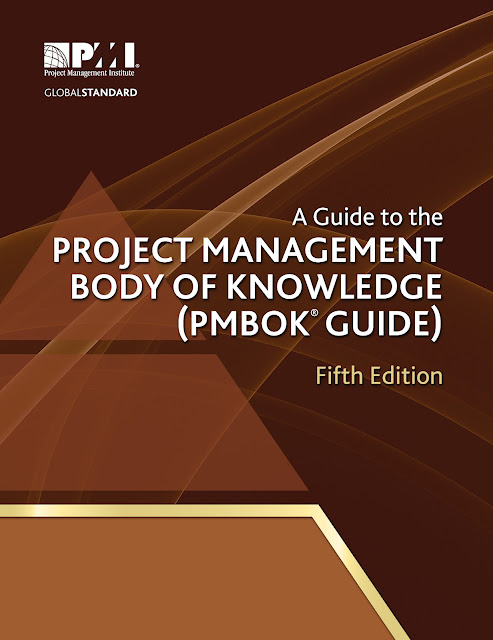
\includegraphics[width = 4cm]{images/book.jpg}
\end{figure}
\end{frame}\begin{center}\line(1,0){250}\end{center}
%% END OF LECTURE SLIDE
 
\subsection{Manage Project Team}
 
 

\begin{frame}
\frametitle{Manage Project Team}
\textbf{Part of the Monitoring and Controlling Process Group}
\begin{figure}
	\centering
		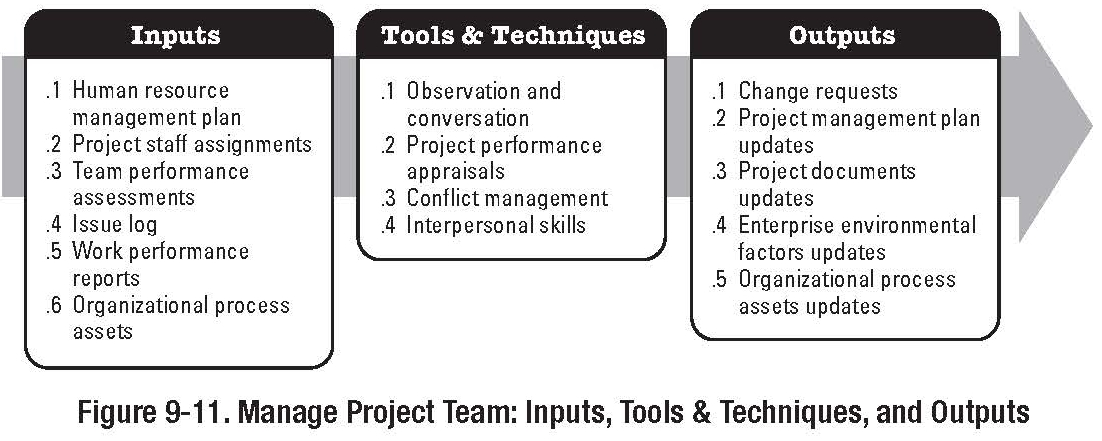
\includegraphics[width = 10cm]{images/Fig9-11.jpg}
	\label{fig:9-11}
\end{figure}
\end{frame}\begin{center}\line(1,0){250}\end{center}
 
 
\begin{frame}
\frametitle{Manage Project Team}
\textbf{Involves:}
\begin{itemize}
	\item Tracking Team Member performance
	\item Providing Feedback
	\item Resolving Issues
	\item Coordinating Change
\end{itemize}
\end{frame}\begin{center}\line(1,0){250}\end{center}


\begin{frame}
\frametitle{Manage Project Team \hfill Inputs}
\textbf{Organisational Process Assets}
	\begin{itemize}
		\item Organisations policies, procedures and systems for rewarding employees
	\end{itemize}
\textbf{Project Staff Assignments}
	\begin{itemize}
		\item Refer to book and previous lectures
	\end{itemize}
\textbf{Staffing Management Plan}
	\begin{itemize}
		\item Refer to book and previous lectures
	\end{itemize}
\end{frame}\begin{center}\line(1,0){250}\end{center}
 
 
\begin{frame}
\frametitle{Manage Project Team \hfill Inputs}
\textbf{Team Performance Assessment}
\begin{itemize}
	\item Formal and Informal assessment of team performance.
	\begin{itemize}
		\item Good PM will identify and resolve issues and potential issues early
	\end{itemize}
	\item Work Performance Information
	\begin{itemize}
		\item PM team directly observes Project Team Performance: Team Member participation in meetings; Follow-up on actions; Communications; Etc.
	\end{itemize}
\end{itemize}
\end{frame}\begin{center}\line(1,0){250}\end{center}
 
 
\begin{frame}
\frametitle{Manage Project Team \hfill Inputs}
\textbf{Performance Reports}
\begin{itemize}
	\item Refer to Section 10; Project Communications Management and EVMS, Comparison between actual and planned progress, etc.
\end{itemize}
\end{frame}\begin{center}\line(1,0){250}\end{center}


\begin{frame}
\frametitle{Manage Project Team \hfill Tools and Techniques}
\textbf{Observation and Conversation}
	\begin{itemize}
		\item Keeps PM in touch with work and attitudes of project team members
	\end{itemize}
\textbf{Project Performance Appraisals}
	\begin{itemize}
		\item Formal and Informal
		\item 360 degree feedback - controversial
		\item Re-clarification of Roles and Responsibilities
	\end{itemize}
\textbf{Conflict Management}
\textbf{Issue Log}
\end{frame}\begin{center}\line(1,0){250}\end{center}


\begin{frame}
\frametitle{Manage Project Team \hfill Tools and Techniques}
\textbf{Conflict Management:}\\
Sources of Conflict
		\begin{enumerate}
			\item Scarce Resources
			\item Scheduling Priorities
			\item Personal Work styles
		\end{enumerate}
\begin{block}{}
Differences of opinion can be healthy, but need to be monitored and controlled in order to avoid creating a negative atmosphere.  Most conflicts amongst team members will resolve themselves.  PM needs to monitor, and may have to facilitate resolution.
\end{block}
\end{frame}\begin{center}\line(1,0){250}\end{center}




\begin{frame}
\frametitle{Manage Project Team \hfill Tools and Techniques}
\textbf{Issue Log}
\begin{itemize}
	\item Refers to recording project team management issues as they arise.
	\item If using this technique, be very careful with the information recorded.  A benign phrase about one person, when taken out of context, can have disastrous effects
	\item Better to keep records to issues of unanticipated responsibilities for future `lessons learned'
\end{itemize}
\end{frame}\begin{center}\line(1,0){250}\end{center}



\begin{frame}
\frametitle{Manage Project Team \hfill Outputs}
\textbf{Change Requests}
\begin{itemize}
	\item Sent through the Integrated Change Control Process
	\item Recommended Corrective Actions
			\begin{itemize}
				\item Staffing Changes\\
				\item Additional Training\\
				\item Disciplinary Actions\\
			\end{itemize}

	\item Recommended Preventative Actions\\
			\begin{itemize}
				\item Solve issues before they arise, may require additional training; cross training, clarification of roles, responsibility, authority, etc.
			\end{itemize}
\end{itemize}			
\end{frame}\begin{center}\line(1,0){250}\end{center}
 
 
\begin{frame}
\frametitle{Manage Project Team \hfill Outputs}
\textbf{Organisational Process Assets (Updates)}\\
\begin{itemize}
	\item Input to organisational performance appraisals
		\begin{itemize}
			\item Project Staff should be prepared to provide input for performance appraisal of any project team member with whom they interact in a significant way.  Needs to be treated with caution
		\end{itemize}
	\item Lessons Learned documentation
\end{itemize}
\textbf{Organisation Charts, Position Descriptions, Staffing Management Plans etc.}\\
\textbf{Project Management Plan (Updates)}\\
\end{frame}\begin{center}\line(1,0){250}\end{center}
 
 
\begin{frame}
\frametitle{Project HR Management \hfill Project Manager as a Leader}
\textbf{3 elements of leadership:}
\begin{enumerate}
	\item The person leading
	\item The people being led
	\item The situation (i.e. the project environment)
\end{enumerate}
\textbf{Democratic or Participative Leadership}
\begin{itemize}
	\item PM encourages involvement in decision making
\end{itemize}
\textbf{Laisse-Faire Leadership}
\begin{itemize}
	\item PM turns things over to the project team.. 
\end{itemize}
\textbf{Autocratic Leadership}
\begin{itemize}
	\item PM focuses on tasks with little or no consideration for those performing the work
\end{itemize}
\end{frame}\begin{center}\line(1,0){250}\end{center}
 
 
\begin{frame}
\frametitle{Blanchard - Hersey Situational Model of Leadership}
\begin{columns}
			\begin{column}{0.5\textwidth}
				\begin{itemize}
					\item Leadership style changes according to the situation and the level of subordinates competence.
					\item Reasonable model of how good leaders actually behave.
					\item Attributes of subordinates are considered.
					\item Provides framework for subordinate development.
				\end{itemize}
			\end{column}

			\begin{column}{0.5\textwidth}
				\begin{figure}
					\centering
						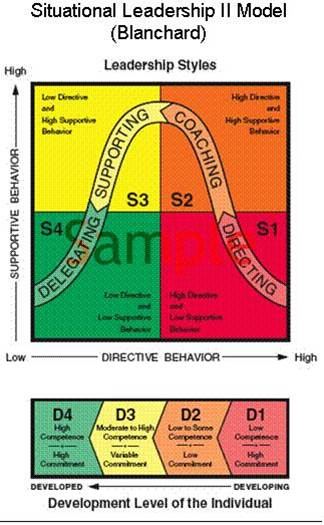
\includegraphics[width = 4cm]{images/bh.jpg}
					\label{fig:blanchard}
				\end{figure}
			\end{column}
\end{columns}
\end{frame}\begin{center}\line(1,0){250}\end{center}



\begin{frame}
\frametitle{Project HR Management \hfill Barriers to Project Team Development}
\begin{enumerate}
	\item Differing outlooks priorities and interests
	\item Role Conflicts
	\item Project objectives/outcomes unclear
	\item Dynamic Project Environment
	\item Competition over team leadership
	\item Lack of team definition and structure
	\item Credibility of project leader
	\item Lack of team member commitment
	\item Communications Problems
	\item Lack of Senior Management Support
\end{enumerate}
\end{frame}\begin{center}\line(1,0){250}\end{center}
 
 
\begin{frame}
\frametitle{Project HR Management}
\textbf{Project Manager pitfalls}
\begin{itemize}
	\item Lack of self-knowledge, ie, your own strengths and weaknesses
	\item Activity traps\\
		\begin{itemize}
			\item  `Means becomes the end' rather than `the means to achieve the end'
		\end{itemize}
	\item Managing versus doing\\
		\begin{itemize}
			\item  Delegating work instead of doing it yourself
		\end{itemize}
	\item	People versus task skills\\
		\begin{itemize}
			\item  Do you use people you get along with in preference to those who can do the task?
		\end{itemize}
	\item Ineffective communications\\
	\item Time Management\\
	\item Management bottlenecks\\
\end{itemize}
\end{frame}\begin{center}\line(1,0){250}\end{center}

Activity Traps are very problematic; it is the illusion of working on something whilst not actually making any real progress.  Consider a research paper.  The deliverable is a high quality research paper.  In order to meet this deliverable, a considerable amount of reading is required.  If you never get out of the reading/analyzing stage, you will never achieve the deliverable.  Often we see evidence of this in individuals who seem to be constantly working, display clear evidence of a broad level of knowledge, but struggle to turn in quality work.\\

Managers are often quite proficient at the work their subordinates do.  This can occasionally lead to difficulties were managers begin to micro-manage subordinates and/or take on their work entirely.  A good manager will help if they can, guide as opposed to instruct, but most of all, allow subordinates to make mistakes; and then correct them.  

 
 
\begin{frame}
\frametitle{Project HR Management \hfill Effective Time Management}
\begin{itemize}
	\item Delegate
	\item Follow the schedule
	\item Decide fast
	\item Decide who should attend
	\item Learn to say no
	\item Start now
	\item Do the tough part first
	\item Control telephone and email time
	\item Refuse to do the unimportant
\end{itemize}
\end{frame}\begin{center}\line(1,0){250}\end{center}




\begin{frame}
\frametitle{7 Habits of Highly Effective People - Steven Covey}
\begin{enumerate}
	\item Be Proactive
	\item Begin with the end in mind
	\item Put first things first
	\item Think win-win
	\item Seek first to understand and then to be understood
	\item Synergize
	\item Sharpen the saw
\end{enumerate}
\end{frame}\begin{center}\line(1,0){250}\end{center}
 
 
\begin{frame}
\frametitle{Habit 3 - Put first things first}
\begin{figure}
	\centering
		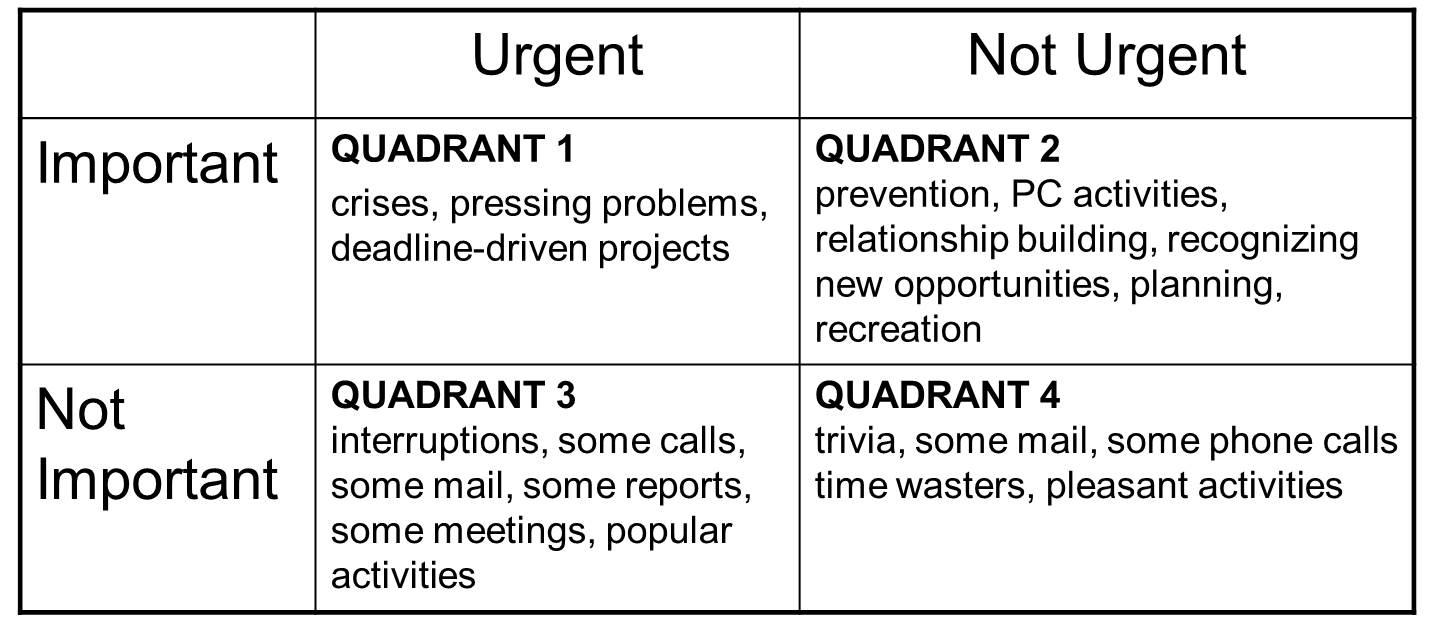
\includegraphics[width = 7cm]{images/habit3.jpg}
	\label{fig:covey}
\end{figure}
\begin{itemize}
	\item The trick is to stay out of Quadrant 3 and 4.
	\item The less time you spend in 3 \& 4 the more time you have for 1 \& 2.
	\item If you work in Quadrant 2, then less activities will end up in Quadrant 1
\end{itemize}
\end{frame}\begin{center}\line(1,0){250}\end{center}
 
\section{Conflict Management, Mediation, Negotiation.}
 
\begin{frame}
\frametitle{Project HR Management}
\textbf{Management of Conflicts}
\begin{itemize}
	\item Study the problem and collect all available information
	\item Develop a situational approach or methodology
	\item Set the appropriate atmosphere or climate
\end{itemize}
\textbf{Confrontation Meeting steps}
\begin{enumerate}
	\item Establish a willingness to participate
	\item Analyse perceptions
	\item Collect Information; get issues out in the open
	\item Define and clarify all problems from both sides
	\item Make information available to both parties
	\item Set priorities for resolution - what is most important to resolve?
	\item Get agreement (or otherwise) and move on
	\item Follow up afterwards
\end{enumerate}
\end{frame}\begin{center}\line(1,0){250}\end{center}
 
 

 
 
 
 
 
\begin{frame}
\frametitle{Project HR Management}
\textbf{Conflict Minimisation Procedures}
\begin{enumerate}
	\item Pause and Think before reacting
	\item Build Trust
	\item Try to understand the conflict motives
	\item Keep the meeting under control
	\item Listen to all involved parties
	\item Maintain a give and take attitude
	\item Tactfully inform others of your view
	\item Be willing to admit when you are wrong
\end{enumerate}
\end{frame}\begin{center}\line(1,0){250}\end{center}
 

\begin{frame}
\frametitle{Project HR Management \hfill Successful Mediation}
\textbf{Selecting the Mediator}
\begin{itemize}
	\item Both parties must be comfortable and trust the mediator to act in an impartial manner
\end{itemize}
\textbf{Preparation for Mediation} 
\begin{itemize}
	\item Do your homework; know everything you can about the issue under dispute
\end{itemize}
\textbf{Commitment}
\begin{itemize}
	\item Both parties need to enter mediation (conciliation) with the intension of resolving the issue
\end{itemize}
\textbf{Authority to Act}
\begin{itemize}
	\item Those attending the meeting must have the authority to negotiate and agree resolution	
\end{itemize}
\textbf{Finality}
\begin{itemize}
	\item Agreement should put the issue to rest.
\end{itemize}
\end{frame}\begin{center}\line(1,0){250}\end{center}



\begin{frame}
\frametitle{Project HR Management \hfill Negotiation}
\begin{itemize}
	\item \textbf{Objectives} 
		\begin{itemize}
			\item Win-Win (ideal)
			\item Win-Lose (problematic)
			\item Lose-Lose (all to often the result)
		\end{itemize}
	\item \textbf{Preparation}
		\begin{itemize}
			\item Analyze Competition (Purchasing)
			\item Information Gathering
			\item Setting Objectives
			\item Selecting Negotiating Team
		\end{itemize}
\end{itemize}
\end{frame}\begin{center}\line(1,0){250}\end{center}

\begin{frame}
\frametitle{Project HR Management \hfill Negotiation}
\textbf{Principles of Negotiation - Persuasion}
\begin{itemize}
	\item Compromise - both parties concede or agree
	\item Bargaining - `trading' options
	\item Coercion - forcing other party to agree (requires power)
	\item Emotion - ``I'm not comfortable with\ldots''
	\item Logical Reasoning - building a solid case to undermine other side
\end{itemize}
\end{frame}\begin{center}\line(1,0){250}\end{center}

 
\begin{frame}
\frametitle{Project HR Management \hfill Negotiation}
\textbf{Principles of Negotiation}
\begin{itemize}
	\item Listening
	\item Creating an atmosphere
	\item Seek Opportunities (Alan Sugar on Sat dishes)
	\item Know the other side and try to understand their position
	\item Assumptions (don't make them)
	\item Question - get answers to assumptions!
	\item Continually summarise current position during negotiations
\end{itemize}
\end{frame}\begin{center}\line(1,0){250}\end{center} 
 



\begin{frame}
\frametitle{Project HR Management \hfill Negotiation}
\textbf{Negotiation Do's}
\begin{itemize}
	\item Prepare
	\item Aim high
	\item Confirm Authority to make decisions
	\item Maintain control - keep questioning and putting points forward
	\item Be professional -joke, gesture, attitude, etc. 
\end{itemize}
\end{frame}\begin{center}\line(1,0){250}\end{center} 



\begin{frame}
\frametitle{Project HR Management \hfill Negotiation}
\textbf{Negotiation Dont's}
\begin{itemize}
	\item Give unnecessary information
	\item Assume anything
	\item Get uncomfortable with silence (pregnant pause)
	\item Give agreement signals (nodding, etc.)
	\item Negotiate with something you don't have
\end{itemize}
\end{frame}\begin{center}\line(1,0){250}\end{center} 







\begin{frame}
\frametitle{Project HR Management \hfill Negotiation}
\textbf{Closing Down}
\begin{itemize}
	\item Confirm Agreement in detail
	\item Allow all parties closing statements
	\item Debrief Negotiation Team (What worked, what didn't, what to do next, etc.)
\end{itemize}
\end{frame}\begin{center}\line(1,0){250}\end{center} 




\begin{frame}
\frametitle{Project HR Management \hfill Negotiation}
\begin{figure}[htbp]
	\centering
		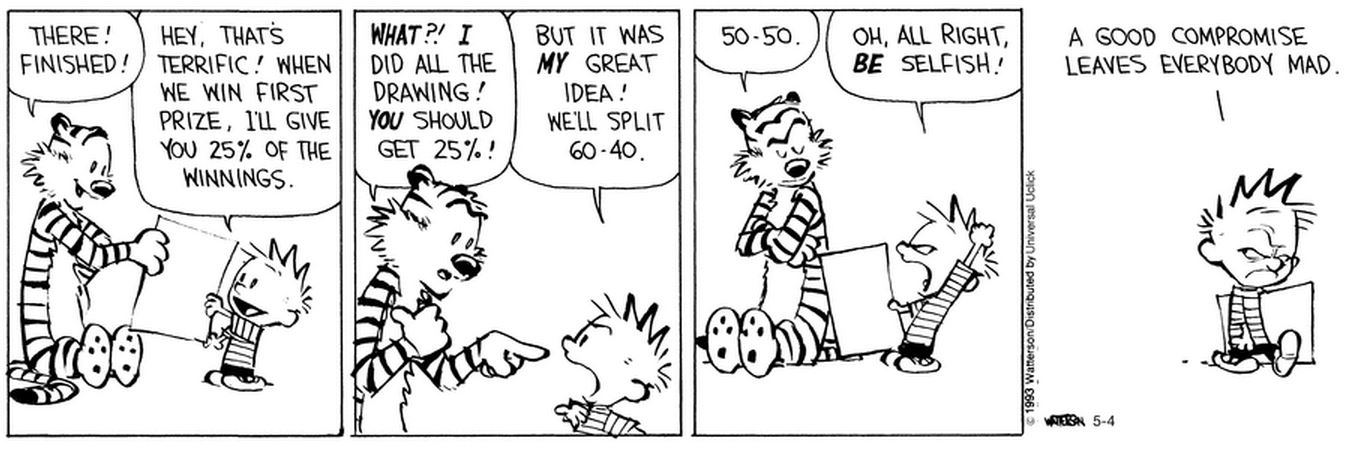
\includegraphics[width=10cm]{images/candh.JPG}
	\caption{Calvin \& Hobbs - Bill Waterson}
	\label{fig:candh}
\end{figure}
\end{frame}\begin{center}\line(1,0){250}\end{center} 


A good compromise leaves everybody mad.  It is useful to know that there are times when resolution of the conflict is not the goal of all parties.  A typical dispute management clause in a contract involves steady escalation; i.e. Conciliation, then Arbitration.  One party may enter conciliation wanting to put the issue in front of an arbitrator.  Why you may ask?  There are cases where the outcome from one project will have an impact on a similar project not under dispute.  As the arbitration judgment is made by an independent third party it is a good indication of how a similar dispute will be handled on another project.  Historically, there was a third stage; the High Court.  Attempts to overturn arbitrators decisions are rare in the High Court now since Limerick City Council v Uniform Construction Limited [2005] IEHC 347. A recent attempt by Dunnes Stores also failed\\
\href{http://www.courts.ie/judgments.nsf/6681dee4565ecf2c80256e7e0052005b/8eda0a6f7c2422988025714d0056fb44?OpenDocument}{Limerick City Council v Uniform Construction Limited}\\
\href{http://courts.ie/Judgments.nsf/09859e7a3f34669680256ef3004a27de/9316804eb3eee080802579ce00517325?OpenDocument}{Dunnes Stores v Holtgen Ltd}\\


%% END OF LECTURE SLIDE
\begin{frame}
\frametitle{Next Lecture \hfill Reading:}
`A Guide to the Project Management Body of Knowledge'\\ 
Chapter 11
\begin{figure}[h]
	\centering
		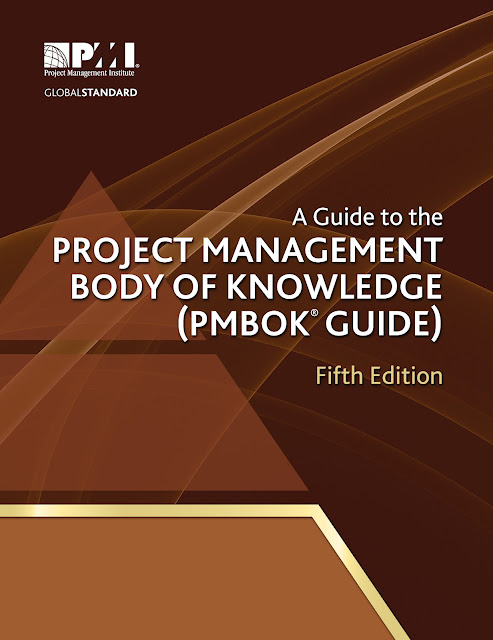
\includegraphics[width = 4cm]{images/book.jpg}
\end{figure}
\end{frame}\begin{center}\line(1,0){250}\end{center}
%% END OF LECTURE SLIDE





\end{document}
